
% Tiers, Dynamic reconfiguration, Peer-to-peer, Publish-subscribe

%1
\newcommand{\qPeerToPeerSpace}{
\begin{ClosedQuestion}
	The Peer-to-Peer architectural style provides high scalability and availability. In the context of a file sharing system  
	

    \optionA{The file transfers follows the same path of nodes used to identify where the file was located.}
    \optionB{The peer initiating the request for a file needs to know where the file is located.}
    \optionC{If a peer providing a file crashes it is necessary to restart to download the file from the begin.}
    \optionD{The price for high scalability and availability is the need to have several replicas of the files to be shared.}
 \putOptions
\end{ClosedQuestion}
}

%2
\newcommand{\qPeerToPeerDynamicReconfiguration}{
\begin{ClosedQuestion}
	In the description of the Gnutella system can be read:
	
	\begin{quote}
		The topology of the system changes at runtime as peer components connect and disconnect to the network.
	\end{quote}
	

    \optionA{When a peer connects to the network it establishes connections with all other peers in the network.}
    \optionB{The behavior described in the sentence can be represented in a view where the dynamic reconfiguration architectural style is used.}
    \optionC{When a peer receives a connection it sends all its files to the peer connecting it.}
    \optionD{The behavior described in the sentence can be represented in a view where the tier architectural style is used.}
 \putOptions
\end{ClosedQuestion}
}

%3
\newcommand{\qTiers}{
\begin{ClosedQuestion}
	The Tiers architectural style
	

    \optionA{It applies layers to tiers.}
    \optionB{Restrict the communication between components because, for instance, a group of components should be located in the same hardware.}
    \optionC{Is an extension of the Client-Server architectural style.}
    \optionD{Defines tiers as components.}
 \putOptions
\end{ClosedQuestion}
}

%4
\newcommand{\qPublishSubscribe}{
\begin{ClosedQuestion}
	In the Publish-Subscribe architectural style 
	

    \optionA{A component can subscribe to events.}
    \optionB{All the published events are received by their subscribing components.}
    \optionC{The events should be delivered by the same order they are sent.}
    \optionD{The set of events types are predefined at initialization time.}
 \putOptions
\end{ClosedQuestion}
}


% SOA, Pipes-and-Filters

%5 
\newcommand{\qSOAInteroperability}{
\begin{ClosedQuestion}
	The Service-Oriented Architecture style improves interoperability because
	

    \optionA{It enforces the use of a single implementation language among all applications.}
    \optionB{The orchestration is in charge of improving the transparent location of service providers.}
    \optionC{The enterprise service bus coordinates the execution of several services.}
    \optionD{It decouples applications developed for different organizations.}
 \putOptions
\end{ClosedQuestion}
}

%6 
\newcommand{\qSOAQualities}{
\begin{ClosedQuestion}
	The Service-Oriented Architecture style improves modifiability because
	

    \optionA{It encapsulates applications through well-defined interfaces.}
    \optionB{It decouples the coordination of the interaction among applications from the applications themselves.}
    \optionC{It improves transparency of location of service providers.}
    \optionD{It encapsulates applications through well-defined interfaces, decouples the coordination of the interaction among applications from the applications themselves, and improves transparency of location of service providers.}
 \putOptions
\end{ClosedQuestion}
}

%7
\newcommand{\qSOAClientServerPeertoPeer}{
\begin{ClosedQuestion}
	The Service-Oriented Architecture style
	

    \optionA{Is a Client-Server style because consumers are clients and providers are servers.}
    \optionB{Is a Peer-to-Peer style because consumers and providers are peers.}
    \optionC{Can use a Service Registry to improve transparency of location of service providers.}
    \optionD{Is a Publish-subscriber style because consumers use an enterprise service bus.}
 \putOptions
\end{ClosedQuestion}
}

%8
\newcommand{\qPipeFilterComposition}{
\begin{ClosedQuestion}
	The Pipe-and-Filter style allows composition of filters 
	

    \optionA{But when the filters are executed sequentially the composition power is reduced.}
    \optionB{Which improves modifiability, because filters are decoupled through pipes.}
    \optionC{But the size of buffers may reduce the composition power.}
    \optionD{And filters do not have to agree on the data formats.}
 \putOptions
\end{ClosedQuestion}
}

% Graphite views

%9
\newcommand{\qGraphiteDecompositionMemcached}{
\begin{ClosedQuestion}
	Consider the following decomposition view of the Graphite system where module \textsc{Store Graphs} is responsible for managing the storage of datapoints and graphs and module \textsc{Present Graphs} for graphs generation and presentation. Memcache is a library that maintains datapoints in memory to reduce the overhead of obtaining them from the file system.
	
	\centering
	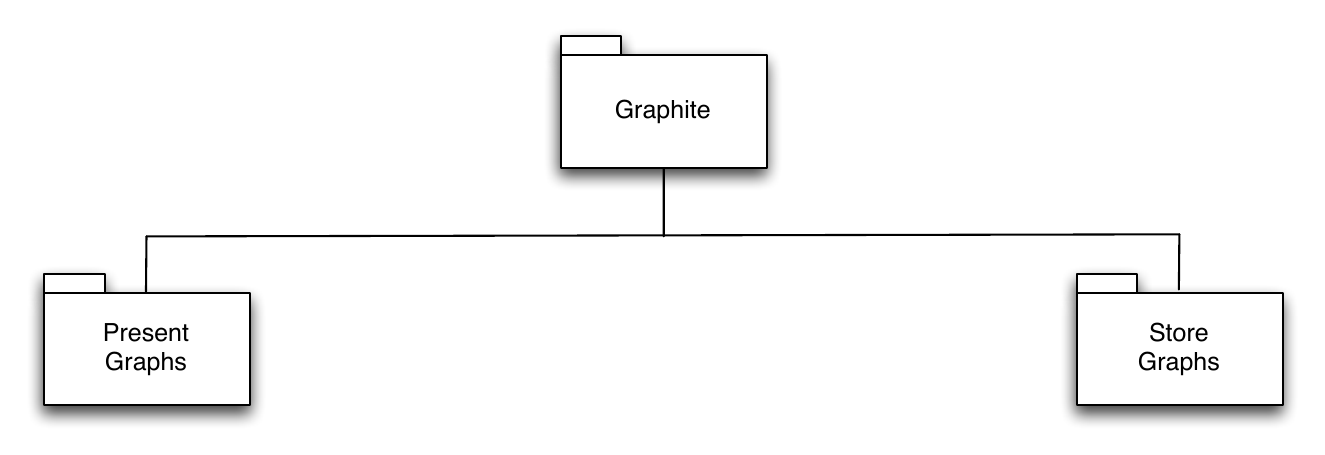
\includegraphics[width=100mm]{x-top-decomposition}

    \optionA{Memcached can be considered a sub-module of the Store Graphs module.}
    \optionB{Memcached can be considered a sub-module of the Present Graphs module.}
    \optionC{Memcached can be considered a direct sub-module of the top Graphite module.}
    \optionD{Memcached is not a module.}
 \putOptions
\end{ClosedQuestion}
}

%10
\newcommand{\qGraphiteDecompositionBuffering}{
\begin{ClosedQuestion}
	Consider the following decomposition view of the Graphite system where module \textsc{Store Graphs} is responsible for managing the storage of datapoints and graphs and module \textsc{Present Graphs} for graphs generation and presentation. Buffering is a library used to temporarily store incoming data point.
	
	\centering
	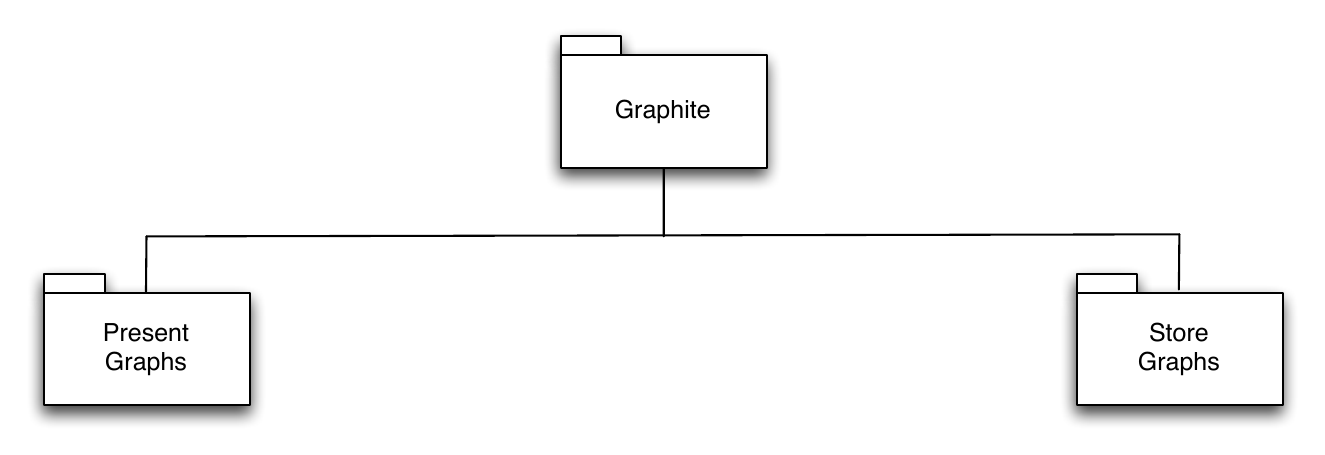
\includegraphics[width=100mm]{x-top-decomposition}

    \optionA{Buffering can be considered a sub-module of the Store Graphs module.}
    \optionB{Buffering can be considered a sub-module of the Present Graphs module.}
    \optionC{Buffering can be considered a direct sub-module of the top Graphite module.}
    \optionD{Buffering is not a module.}
 \putOptions
\end{ClosedQuestion}
}

%11
\newcommand{\qGraphiteCarbon}{
\begin{ClosedQuestion}
	Consider the following application-specific types that were defined for a component-and-connector view that depicts the components within \texttt{Carbon} component. 
	
	\centering
	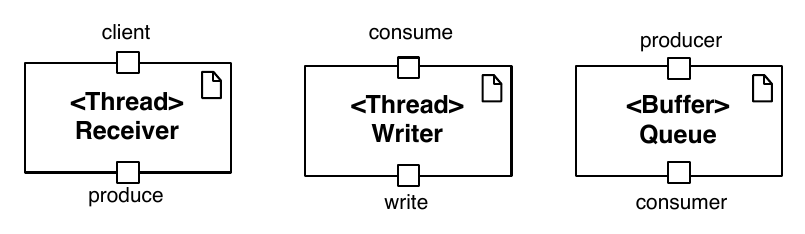
\includegraphics[width=100mm]{x-carbon-buffering}

    \optionA{In the view there are multiple instances of the \texttt{Queue} component.}
    \optionB{In the view there are multiple instances of the \texttt{Writer} component.}
    \optionC{In the view \texttt{Receiver} component's \texttt{client} port is not associated with an external port.}
    \optionD{In the view the \texttt{produce} port of a \texttt{Receiver} component is attached to the \texttt{consume} port of a \texttt{Writer} component.}
 \putOptions
\end{ClosedQuestion}
}


%12
\newcommand{\qGraphiteDataPointSocket}{
\begin{ClosedQuestion}
	Consider the following application-specific types. Note that \texttt{Queue} components are within the \texttt{Carbon} components. In a view that contains components of these three types 
	
	\centering
	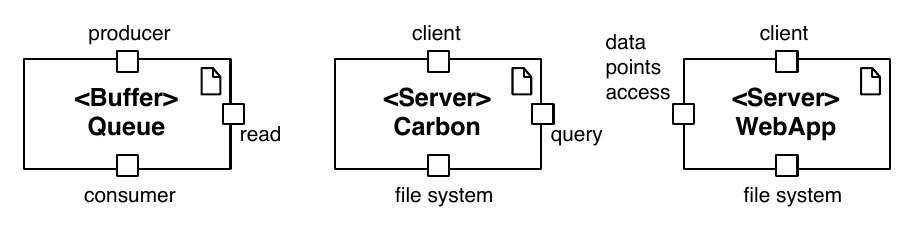
\includegraphics[width=120mm]{x-datapoint-access}

    \optionA{There is a message passing connector between the \texttt{read} port of \texttt{Queue} and the \texttt{data points access} port of \texttt{WebApp}.}
    \optionB{There is a interface delegation relation between the \texttt{read} port of \texttt{Queue} and the \texttt{query} port of \texttt{Carbon}.}
    \optionC{There is a connector between the \texttt{producer} port of a \texttt{Queue} component and the \texttt{client} port of its \texttt{Carbon} component.}
    \optionD{The \texttt{client} ports of \texttt{Carbon} and \texttt{WebApp} are connected to a \texttt{Client} component through the same connector instance.}
 \putOptions
\end{ClosedQuestion}
}


% Allocation viewtype

%13
\newcommand{\qAllocationStylesCost}{
\begin{ClosedQuestion}
	Consider a stakeholder that is particularly concerned about the total cost of the project. When it comes to describing the system using allocation viewtypes is interested in

    \optionA{A deployment view.}
    \optionB{A work assignment view.}
    \optionC{A deployment and a work assignment view.}
    \optionD{A install view.}
 \putOptions
\end{ClosedQuestion}
}

%14
\newcommand{\qImplementationStyle}{
\begin{ClosedQuestion}
	An architecture can also be represented by the set of files which contains its modules code. A suitable architectural style to represent this set of files is

    \optionA{Deployment style.}
    \optionB{Implementation style.}
    \optionC{Install style.}
    \optionD{Work assignment style.}
 \putOptions
\end{ClosedQuestion}
}

%15
\newcommand{\qInstallStyle}{
\begin{ClosedQuestion}
	An important stage of the development of any system is its build into the set of executable files. A suitable architectural style which helps on the definition of the build process is

    \optionA{Deployment style.}
    \optionB{Implementation style.}
    \optionC{Install style.}
    \optionD{Work assignment style.}
 \putOptions
\end{ClosedQuestion}
}

%16
\newcommand{\qDeploymentStyleLimitExposure}{
\begin{ClosedQuestion}
	An architect needs to show that a security tactic of limit exposure will be effectively provided by the executing system. Therefore, she decides to design
	
    \optionA{A work assignment view.}
    \optionB{A deployment view.}
    \optionC{An install view.}
    \optionD{An implementation view.}
 \putOptions
\end{ClosedQuestion}
}


% DVD Catalog

%17
\newcommand{\qDVDCatalogMeta}{
\begin{ClosedQuestion}
	Consider the module viewtype views of the DVDCatalog application. The architect knows about a new requirement 
	
	\begin{quote}
		The application should support other kinds of catalogs (CDs, games, books, ...). 
	\end{quote}
	
	This requirement requires a change of
	
    \optionA{The layered view to support a new specific layer for the customization of the catalog.}
    \optionB{The layered view to accommodate a new layer for which kind of catalog, which other layers may use.}
    \optionC{The data model view in order to define entities for each kind of catalog.}
    \optionD{The data model view in order to define generic entities that can be customized for different kinds of catalogs.}
 \putOptions
\end{ClosedQuestion}
}

%18
\newcommand{\qDVDCatalogAspects}{
\begin{ClosedQuestion}
	Consider the module viewtype views of the DVDCatalog application. The architect knows about a new requirement 
	
	\begin{quote}
		To allow the share of catalogs with family and friends, including some access control. 
	\end{quote}
	
	This requirement requires 
	
    \optionA{A change to the uses view to represent that friends can use each other catalog.}
    \optionB{A change of the layered view to support different presentations, one for each friend.}
    \optionC{A change of the decomposition view to include the responsibilities associated with the access control.}
    \optionD{A new aspect view to include the responsibilities associated with the access control.}
 \putOptions
\end{ClosedQuestion}
}

%19
\newcommand{\qDVDCatalogMobile}{
\begin{ClosedQuestion}
	Consider the module viewtype views of the DVDCatalog application. The architect knows about a new requirement 
	
	\begin{quote}
		To support iPhone/iPad/Android version with sync, which allows offline use of the application in the mobile device and data synchronization to occur when a connection is available
	\end{quote}
	
	This requirement requires a change of
	
    \optionA{The decomposition view to include a module for the synchronization responsibilities.}
    \optionB{The uses view to represent how the mobile device uses the Catalog application.}
    \optionC{The layered view to include a layer for each type of device.}
    \optionD{The domain layer of the layered view to represent the types of devices.}
 \putOptions
\end{ClosedQuestion}
}

%20
\newcommand{\qDVDCatalogMultiPlatform}{
\begin{ClosedQuestion}
	Consider the module viewtype views of the DVDCatalog application. The architect knows about a new requirement 
	
	\begin{quote}
		To support multi-platform (Mac, Windows, Linux)
	\end{quote}
	
	This requirement requires a change of
	
    \optionA{The layered view to deal with the aspects of portability.}
    \optionB{The uses view to show the coupling between the different platforms.}
    \optionC{The uses view to show the uses relationships between the different platforms.}
    \optionD{The data model view to represent each one of the platforms.}
 \putOptions
\end{ClosedQuestion}
}


